\documentclass[aspectratio=169, 11pt]{beamer}

\usetheme{Madrid}
\usecolortheme{default}
\usefonttheme{professionalfonts}

\usepackage{amsmath, amssymb, amsthm}
\usepackage{graphicx}
\usepackage{booktabs}
\usepackage{xcolor}

\definecolor{darkblue}{RGB}{0,51,102}

\setbeamercolor{frametitle}{bg=darkblue, fg=white}
\setbeamercolor{title}{fg=darkblue}
\setbeamercolor{structure}{fg=darkblue}
\setbeamertemplate{navigation symbols}{}
\setbeamertemplate{footline}[frame number]

\newcommand{\IC}{\mathrm{IC}}
\newcommand{\SNR}{\mathrm{SNR}}
\newcommand{\GP}{\mathcal{GP}}
\newcommand{\Nrm}{\mathcal{N}}
\newcommand{\Hk}{\mathcal{H}}
\newcommand{\R}{\mathbb{R}}
\newcommand{\E}{\mathbb{E}}
\newcommand{\Var}{\operatorname{Var}}

\title{\textcolor{white}{Modeling the Dynamic Conditional Information Coefficient}}
\subtitle{Kernel Methods for Equity Return Prediction in Low-SNR Environments}
\author{Conner B.\ Draper \and Seokkwon Yoon}
\date{Math 404}

\begin{document}

% ── 1. TITLE ──────────────────────────────────────────────────────────────────
\begin{frame}
  \titlepage
\end{frame}

% ── 2. SETUP ──────────────────────────────────────────────────────────────────
\begin{frame}{Setup}
  \textbf{Goal.} Predict next-day stock return $r_{i,t+1}$ from a signal $z_{i,t}$ (cross-sectional z-score).

  \bigskip
  \textbf{Standard model} (Grinold \& Kahn, 1999):
  \[
    \E[r_{i,t+1} \mid z_{i,t}] = \IC \cdot \sigma_{i,t} \cdot z_{i,t}
  \]
  $\IC$ = correlation between signal and returns.
  Think of it as \emph{scaled confidence}: $\IC \approx 0.05$ means the signal is right $\sim$52\% of the time.

  \bigskip
  \textbf{Our extension.} Condition IC on $z$ and let it drift over time:
  \[
    \E[r_{i,t+1} \mid z_{i,t}] = \IC_t(z_{i,t}) \cdot \sigma_{i,t} \cdot z_{i,t}
  \]
  We estimate $\IC_t(\cdot)$ with kernel regression on a rolling 504-day window.

  \bigskip
  \textbf{Motivation.} The assumption that IC=$+0.05$ for all signals, across all time is an gross oversimplification.
  IC is likely a non-linear function of $z$ that decays to 0 time.
\end{frame}

% ── 3. DATA ───────────────────────────────────────────────────────────────────
\begin{frame}{Data}
  \begin{columns}
    \begin{column}{0.33\textwidth}
      Barra U.S.\ equity model, 1995--2025\\[6pt]
      ${\sim}3{,}000$ stocks/day\\[6pt]
      \textbf{8 signals:}
      \begin{itemize}
        \item Style / industry / idiosyncratic momentum
        \item Style / industry / idiosyncratic reversal
        \item Idiosyncratic volatility
        \item Betting-against-beta
      \end{itemize}
      \vspace{6pt}
      We regress on $y_{i,t} = r_{i,t+1}/\sigma_{i,t}$\\
      so OLS slope $=$ IC directly.
    \end{column}
    \begin{column}{0.65\textwidth}
      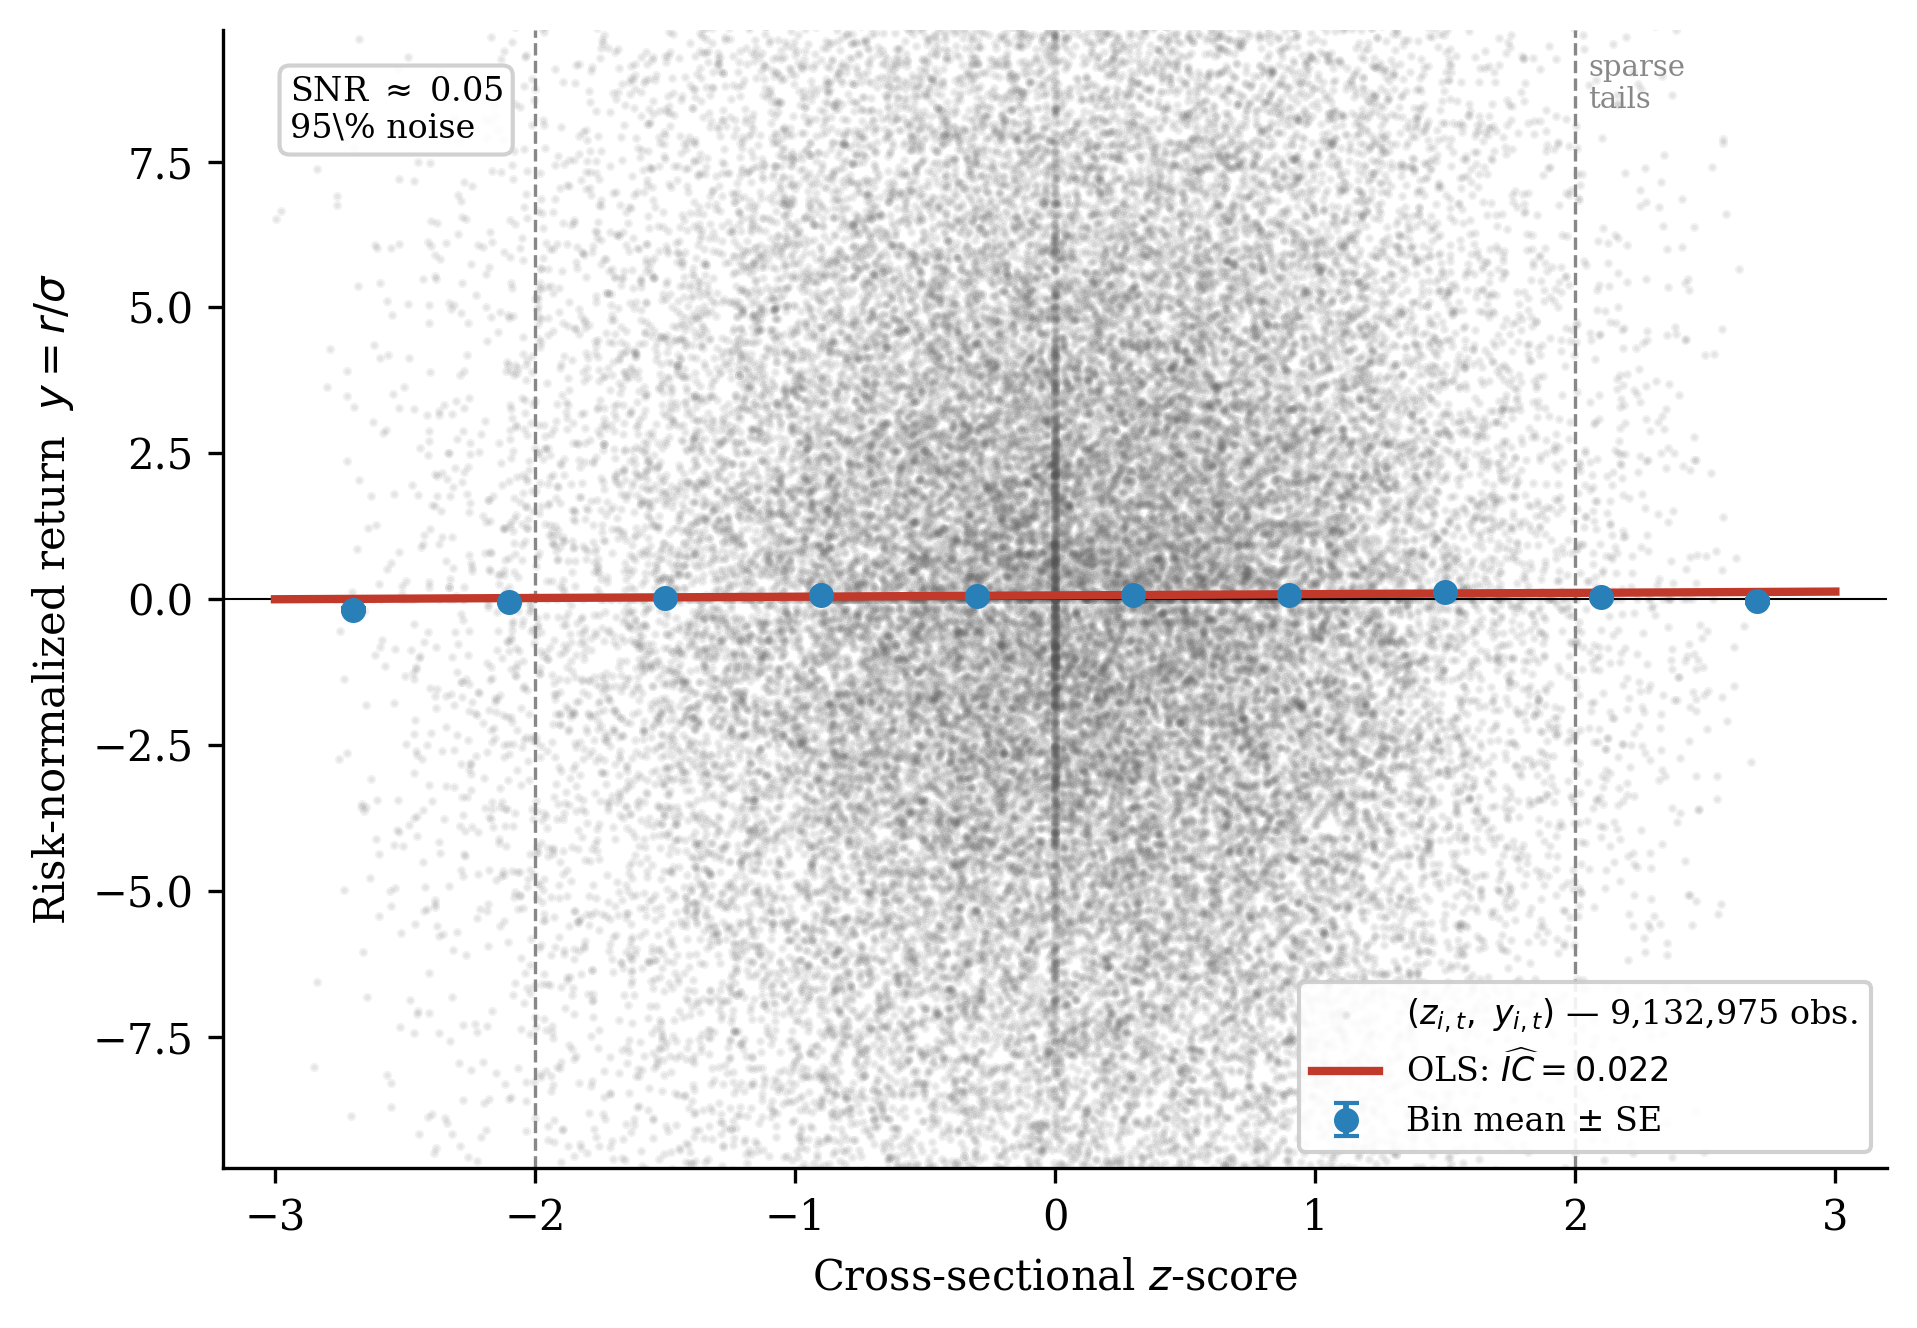
\includegraphics[width=\linewidth]{blob_chart.png}\\[-2pt]
      {\footnotesize
        Style momentum signal pooled across all stocks and dates (1995--2025).
        Red line: OLS $\widehat{\IC}\approx 0.05$.
      }
    \end{column}
  \end{columns}
\end{frame}

% ── 4. METHODS: KRR ───────────────────────────────────────────────────────────
\begin{frame}{Kernel Ridge Regression (KRR)}
  \textbf{Mathematical Core.} Learn $f\colon\R\to\R$ via regularized least squares in an RKHS:
  \[
    \min_{f\in\Hk}\;\sum_{i=1}^n(f(z_i)-y_i)^2 + \alpha\|f\|_\Hk^2
  \]

  \textbf{Update Step (Daily Training).}
  \begin{itemize}
    \item \textbf{Buffer:} Maintain a rolling 504-day window of cross-sectional $(z, y)$ pairs.
    \item \textbf{Fit:} Heavy regularization $\alpha \approx 19$ (Noise-to-Signal ratio) forces high-bias/low-variance predictions to suppress noise.
  \end{itemize}

  \textbf{Predict Step (Inference).}
  \begin{itemize}
    \item Input today's $z$-scores. Because $y_i \approx \IC \cdot z_i$, the model outputs $\alpha_z = \widehat{\IC}(z) \cdot z$ directly.
    \item Output is unconstrained in sign, natively capturing negative IC.
    \item Uncertainty (variance) is treated as a static heuristic based on $\alpha$.
  \end{itemize}
\end{frame}

% ── 5. METHODS: GPR ───────────────────────────────────────────────────────────
\begin{frame}{Gaussian Process Regression (GPR)}
  \textbf{Mathematical Core.} Bayesian prior over functions $f\sim\GP(0,k)$.
  Kernel: $k(z,z') = \text{Constant} \times \text{RBF} + \text{WhiteKernel}$.

  \textbf{Update Step.}
  \begin{itemize}
    \item Uses the exact same 504-day rolling buffer and 300-point recent subsample as KRR.
    \item \textbf{Fit:} WhiteKernel noise is \emph{fixed} at 0.95 (representing 95\% noise). This forces the exact posterior to ignore daily volatility and focus on smooth, persistent trends.
  \end{itemize}

  \textbf{Predict Step.}
  \begin{itemize}
    \item Output yields expected return $\mu_*(z)$ AND predictive variance $\sigma_*^2(z)$.
    \item \textbf{Key advantage:} Provides dynamic, point-wise uncertainty useful for downstream portfolio sizing (unlike KRR's flat variance).
  \end{itemize}

  % \textbf{Calibration Note.} GPR's effective regularization ($\approx 0.95$) is roughly $\mathbf{20\times}$ \textbf{weaker} than KRR's ($\alpha \approx 19$). Despite this, GPR outperforms (Sharpe 2.40 vs.\ 1.85), suggesting true IC is more learnable than the $0.05$ SNR implies for the signals where GPR wins.
\end{frame}

% ── 6. PORTFOLIO CONSTRUCTION ─────────────────────────────────────────────────
\begin{frame}{Portfolio Construction}
  \textbf{Alpha forecast:}
  \[
    \hat\alpha_{i,t} = \widehat{\IC}_t(z_{i,t})\cdot\sigma_{i,t}\cdot z_{i,t}
  \]

  \bigskip
  \textbf{Optimization.} Mean-variance optimization converts alphas into weights.
  Constraints: dollar-neutral (equal long/short) and market-neutral (zero net beta).
  Returns reflect pure signal skill with no directional market exposure.

  \bigskip
  \textbf{Pipeline.}
  \begin{enumerate}
    \item Each of the 8 signals runs through its own model independently
    \item Each produces a daily long-short portfolio
    \item Final portfolio = equal-weight average of all 8
  \end{enumerate}
  Walk-forward: fit on past 504 days $\to$ predict $\to$ optimize $\to$ trade. No lookahead.
\end{frame}

% ── 7. RESULTS: MOE CHART ─────────────────────────────────────────────────────
\begin{frame}{Results: Mixture of Experts (1995--2025)}
  \begin{center}
    \includegraphics[width=0.88\linewidth]{../results/full/performance_moe_portfolio.png}
  \end{center}
\end{frame}

% ── 8. RESULTS: TABLE ─────────────────────────────────────────────────────────
\begin{frame}{Results: Portfolio Comparison}
  \textbf{Mixture of Experts}: for each signal, pick the model with the highest Sharpe,
  then equal-weight the 8 winners.
  GPR wins 6 of 8 signals. Static wins idiosyncratic reversal and volatility (signals
  with the most stable, linear IC).

  \bigskip
  \begin{center}
  \renewcommand{\arraystretch}{1.5}
  \begin{tabular}{lcccc}
    \toprule
    \textbf{Portfolio} & \textbf{Cum.\ Return \%} & \textbf{Ann.\ Return \%} & \textbf{Sharpe} & \textbf{Max DD \%} \\
    \midrule
    \textbf{MoE} (best model per signal) & $\mathbf{97.9}$ & $\mathbf{3.33}$ & $\mathbf{4.34}$ & $-2.61$ \\
    Static (EW all signals)              & $74.7$          & $2.54$          & $3.58$          & $-3.20$ \\
    GPR (EW all signals)                 & $39.1$          & $1.33$          & $2.40$          & $-0.87$ \\
    KRR (EW all signals)                 & $26.0$          & $0.89$          & $1.85$          & $-1.13$ \\
    \bottomrule
  \end{tabular}
  \end{center}
\end{frame}

% ── 9. ETHICS ─────────────────────────────────────────────────────────────────
\begin{frame}{Ethical Implications}
  \begin{block}{1. The Zero-Sum Nature of Alpha}
    Short-term alpha generation is essentially a zero-sum game. By executing trades based on predictive signals, the model systematically extracts wealth from less-informed market participants, raising questions about the broader societal value of these transactions.
  \end{block}

  \begin{block}{2. Resource and Information Asymmetry}
    Deploying this strategy requires expensive proprietary data (e.g., Barra risk models) and significant daily compute. This structural barrier widens the wealth gap between institutional and retail investors, transferring returns to the better-equipped.
  \end{block}

  \begin{block}{3. Societal Brain Drain}
    Quantitative finance aggressively recruits top-tier STEM talent by offering highly competitive compensation. This siphons intellectual capital away from critical research areas that may offer higher tangible benefits to the public (e.g., healthcare, engineering, or climate science).
  \end{block}
\end{frame}

% ── 10. CONCLUSIONS ───────────────────────────────────────────────────────────
\begin{frame}{Conclusions}
  \begin{block}{Central finding}
    $\IC_t(z)$ is non-constant. Kernel methods capture this, but the benefit is signal-specific.
  \end{block}

  \bigskip
  \begin{itemize}
    \item \textbf{KRR and GPR are nearly identical} in their predictions; GPR additionally
          provides posterior uncertainty used to size positions
    \item \textbf{Dynamic IC helps most} when IC sign is uncertain (factor-based reversal signals)
    \item \textbf{Static IC wins} when IC is stable and positive (idiosyncratic reversal)
    \item \textbf{Mixture of Experts} routes each signal to its best model: Sharpe $3.58 \to 4.34$
  \end{itemize}
\end{frame}

\end{document}
